\documentclass[10pt,twocolumn]{article}

%% ---------------------------------------------------------------
%%  RDTM / Springer style approximation
%%  Final submission: use the official Springer template from
%%  https://www.springernature.com/gp/authors/campaigns/latex-author-support
%% ---------------------------------------------------------------

\usepackage[T1]{fontenc}
\usepackage{mathptmx}          % Times Roman for text and math
\usepackage[margin=2cm,top=2.5cm,bottom=2.5cm]{geometry}
\usepackage{amsmath,amssymb}
\usepackage{graphicx}
\usepackage{caption}
\usepackage{hyperref}
\usepackage{cite}
\usepackage{setspace}
\usepackage{booktabs}
\usepackage{xcolor}

\hypersetup{
  colorlinks=true,
  linkcolor=blue,
  citecolor=blue,
  urlcolor=blue
}

% Float placement parameters
\renewcommand{\topfraction}{0.95}
\renewcommand{\dbltopfraction}{0.95}
\renewcommand{\textfraction}{0.05}
\renewcommand{\floatpagefraction}{0.85}
\renewcommand{\dblfloatpagefraction}{0.85}

% Remove date
\date{}

% ---------------------------------------------------------------
\begin{document}

% ===================== TITLE PAGE ==============================
\twocolumn[{%
\begin{center}
  {\Large\bfseries Neutrino-Nucleon Structure Functions in Duality and
  DIS Regions}\\[1em]

  {\normalsize
  Alka Singh$^{1,*}$,  Huma Haider$^{1}$,  Stephen Pate$^{2}$  and  Richard Gran$^{3}$
  }\\[0.5em]

  {\small
  \itshape $^1$Department of Physics, Aligarh Muslim University, Aligarh 202002, India\\
  $^2$Department of Physics, New Mexico State University, Las Cruces, NM 88003, USA\\
  $^3$Department of Physics, University of Minnesota Duluth, Duluth, MN 55812, USA}\\[0.5em]

  {\small
  $^*$Corresponding author: \href{mailto:alka33330@gmail.com}{alka33330@gmail.com}
  \quad Tel.: +91-9084012818}\\[0.5em]

  {\small\itshape
  Presented at NuFact 2026, Tsung-Dao Lee Institute,
  Shanghai Jiao Tong University, Shanghai, China, 1 September 2026.\\
  Submitted to: \emph{Radiat.\ Detect.\ Technol.\ Methods} (RDTM),
  Special Issue: NuFact 2026.}

\end{center}
\vspace{1em}

% ===================== ABSTRACT ================================
\noindent\rule{\linewidth}{0.4pt}
\begin{center}{\bfseries Abstract}\end{center}
\noindent
\textbf{Purpose:} Neutrino-nucleon charged-current deep inelastic scattering (DIS) in the transition region ($Q^2 \sim 1$--$4$~GeV$^2$) is critical for neutrino oscillation experiments (DUNE, Hyper-Kamiokande, NOvA, T2K), where perturbative QCD breaks down and non-perturbative hadronic effects become significant. This work constructs a hybrid description of weak structure functions $F_2$ and $xF_3$ across this crossover region, motivated by Bloom--Gilman quark--hadron duality.
\textbf{Methods:} We combine the Regge-inspired CKMT parametrization at low $Q^2$ with the AMU perturbative QCD framework (NLO $+$ target mass corrections $+$ higher-twist effects) at higher $Q^2$. The models are matched at changeover scale $Q_0^2 = 2~\mathrm{GeV}^2$ using two established transition prescriptions: a piecewise linear splice and a smooth sigmoid weighting function. In addition, the sensitivity to modern PDF sets (CT10nlo, CT18NLO, MMHT2014) is investigated for free nucleons.
\textbf{Results:} Linear splicing of unscaled CKMT with AMU generates unphysical kink artefacts in $xF_3$ at low~$x$ due to curvature and normalization differences between the models. The smooth sigmoid weighting ($\Delta = 0.25$~GeV$^2$, AMU with LO+NLO+TMC+HT) restores derivative continuity across the matching boundary; however, a non-monotonic dip persists due to the normalization offset between unscaled CKMT and AMU, which is further deepened when higher-twist corrections are included. Predictions from different PDF sets show notable variation at high~$x$ and low~$Q^2$, converging above the matching scale.
\textbf{Conclusion:} The hybrid framework highlights the necessity of smooth matching and proper normalization across the resonance-to-DIS interface. Extension to nuclear targets and data comparison is ongoing.
\\[0.3em]
\noindent\textbf{Keywords:}
neutrino deep inelastic scattering; weak structure functions;
CKMT parametrization; low-$Q^2$ modelling; quark--hadron duality;
PDF sensitivity\\[0.4em]
\noindent\textbf{Acknowledgements and Funding:}
This work was supported in part by the United States Department of Energy (US DOE) under Grant No.~DE-FG02-94ER40847. A.S.\ acknowledges support from the Department of Physics, Aligarh Muslim University, Aligarh. We thank the CT10nlo, CT18NLO, and MMHT2014 collaboration teams for making their PDF error sets publicly available.\\[0.3em]
\noindent\rule{\linewidth}{0.4pt}
\vspace{1em}
}] % end twocolumn title block

% ===================== SECTION 1 ================================
\section{Introduction}
\label{sec:intro}

Neutrino deep inelastic scattering (DIS) spans three kinematic regimes:
quasi-elastic, resonance, and perturbative DIS.
The few-GeV transition region ($Q^2 \sim 1$--$4$~GeV$^2$) is particularly
challenging: significant event rates for experiments such as NOvA, T2K,
DUNE, and Hyper-Kamiokande occur here, yet no single model covers it
self-consistently~\cite{nuxsec}.

Bloom--Gilman quark--hadron duality~\cite{bloomgilman}, and its extension
to neutrino-induced weak processes~\cite{lalakulich}, provides a
theoretical bridge: resonance peaks, when plotted against the modified
scaling variable
$\omega' = (2M\nu + M^2)/Q^2$,
oscillate around the DIS scaling curve and average to reproduce the DIS
result.
This motivates a systematic matching between low-$Q^2$ empirical
parametrizations and perturbative QCD (pQCD) calculations.

Standard generators such as GENIE~\cite{GENIE} and NuWro~\cite{NuWro} rely on the
Bodek--Yang (BY) prescription~\cite{BY} to extend pQCD into the non-perturbative
region, but BY is tied to GRV98 LO PDFs, preventing propagation of modern PDF
uncertainties, and absorbs TMC and HT effects implicitly.
In this work we construct a hybrid framework using the CKMT
parametrization~\cite{CKMT} at low $Q^2$ and an NLO+TMC+HT
calculation (AMU model) at high $Q^2$, and compare two transition
prescriptions for $F_2$ and $xF_3$ for free nucleons.
Extension to nuclear targets is ongoing.

\begin{figure*}[t]
  \centering
  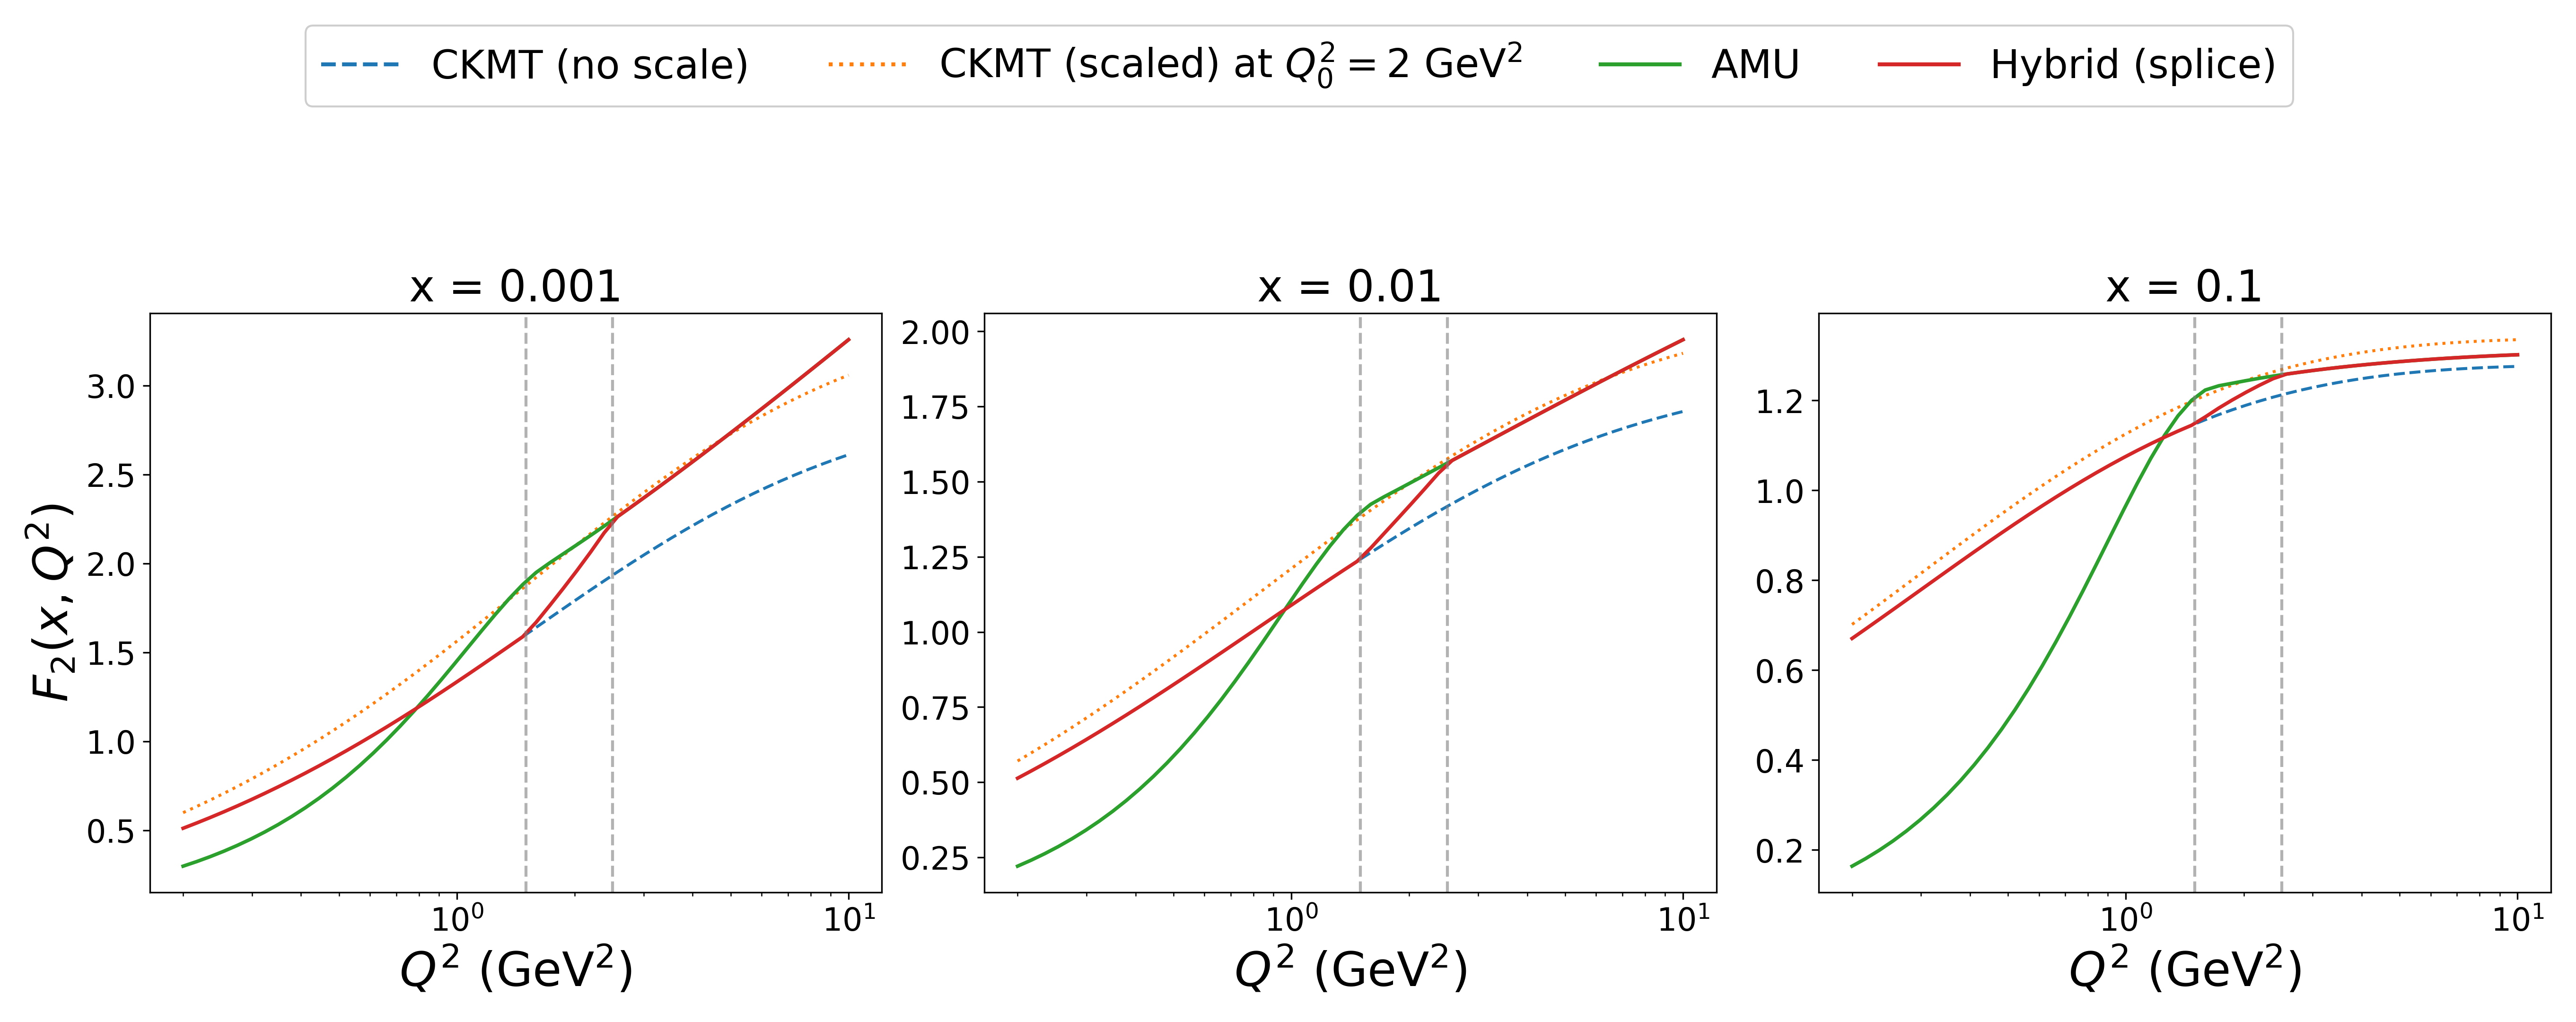
\includegraphics[width=0.75\textwidth]{Fig2.png}
  \caption{$F_2(x,Q^2)$ vs.\ $Q^2$ at $x=0.001, 0.01, 0.1$ for unscaled CKMT (blue dashed),
    scaled CKMT at $Q^2_0=2$~GeV$^2$ (orange dotted), AMU (green solid), and linear splice (red solid).
    Vertical dashed lines mark the splice window $[1.5,\,2.5]$~GeV$^2$.}
  \label{fig:f2_matching}
\end{figure*}

% ===================== SECTION 2 ================================
\section{Theoretical Framework}
\label{sec:theory}

\subsection{Charged-Current DIS Cross Section}

The structure functions $F_2$ and $xF_3$ encode vector and
parity-violating valence quark content respectively; $xF_3$ is particularly
sensitive to the matching prescription since it probes valence quarks
($xF_3^{\nu N} = x[u_v + d_v]$ at leading order)~\cite{jeong}.
For charged-current neutrino scattering
$\nu_\mu(k) + N(p) \to \mu^-(k') + X(p')$, the double-differential
cross section in the laboratory frame is~\cite{jeong}
\begin{equation}
\begin{aligned}
  \frac{d^2\sigma^{\nu,\bar\nu}}{dx\,dy}
  &= \frac{G_F^2 \,M_N E_\nu}{\pi}\left(\frac{M_W^2}{Q^2+M_W^2}\right)^{\!2}
    \biggl[ y^2 x F_1 \\
  &\quad + \!\left(1 - y - \frac{M_N xy}{2E_\nu}\right)\!F_2
    \pm y\!\left(1-\frac{y}{2}\right)\!xF_3 \biggr]\!,
\end{aligned}
  \label{eq:xsec}
\end{equation}
where $x = Q^2/(2M_N\nu)$ is the Bjorken variable, $y = \nu/E_\nu$ is
the inelasticity, $Q^2 = -q^2$ is the momentum transfer squared, $\nu$
is the energy transfer in the lab frame, $M_N$ is the nucleon mass, and
$G_F$ is the Fermi coupling constant. The upper (lower) sign $\pm$ in
Eq.~(\ref{eq:xsec}) applies to neutrino (anti-neutrino) scattering.
\subsection{AMU (High-$Q^2$) Model}

The AMU model computes the structure functions with CT10nlo
PDFs~\cite{CT10}, supplemented by:
\begin{itemize}
  \item \textbf{NLO pQCD}: next-to-leading-order corrections via the
    DGLAP evolution equations.
  \item \textbf{TMC}: Target Mass Corrections following
    Schienbein et al.~\cite{Schienbein}, important at moderate $Q^2$ and
    large~$x$.
  \item \textbf{HT}: Higher Twist corrections
    ($\propto 1/Q^2$), suppressing structure functions at low $Q^2$~\cite{Stein1998,Dasgupta1996}.
\end{itemize}
The AMU model is reliable for $Q^2 \gtrsim 2$~GeV$^2$ but diverges
in the non-perturbative regime.

\subsection{CKMT Parametrization}

The CKMT model~\cite{CKMT} is a Regge-inspired empirical
parametrization originally fitted to electromagnetic $F_2$ data,
which is adapted to charged-current neutrino scattering for both
$F_2^{\rm CC}$ and $xF_3$ following Jeong and Reno~\cite{jeong}.

\subsection{Hybrid Matching: Linear Splice}

To bridge the low-$Q^2$ CKMT regime and high-$Q^2$ pQCD, the two models
are matched across a crossover region around $Q^2_0 = 2.0$~GeV$^2$.
While CKMT can be rescaled to enforce continuity at $Q^2_0$ (``scaled CKMT''),
we preserve the original empirical parametrization (``unscaled CKMT'') in our
hybrid description. A piecewise linear interpolation splice across
$[1.5,\,2.5]$~GeV$^2$ is defined by:
\begin{equation}
  F^{\rm hyb} =
  \begin{cases}
    F^{\rm CKMT}            & Q^2 \le 1.5~\text{GeV}^2,\\[2pt]
    c\,F^{\rm AMU}+(1-c)\,F^{\rm CKMT}
                            & 1.5 < Q^2 < 2.5~\text{GeV}^2,\\[2pt]
    F^{\rm AMU}             & Q^2 \ge 2.5~\text{GeV}^2,
  \end{cases}
  \label{eq:splice}
\end{equation}
with the linear weight $c(Q^2)=(Q^2-1.5)/(2.5-1.5)$.

\subsection{Hybrid Matching: Smooth Sigmoid}

Although the linear splice provides value continuity, differences in
model curvature can induce derivative discontinuities and kink artefacts.
To ensure a continuously differentiable transition, we replace the linear
weight with a smooth sigmoid function, yielding the hybrid structure function:
\begin{equation}
  F^{\rm hyb} = w(Q^2)\,F^{\rm CKMT} + \bigl[1-w(Q^2)\bigr]\,F^{\rm AMU},
  \label{eq:hyb_sig}
\end{equation}
with $w(Q^2) = \tfrac{1}{2}\bigl[1 - \tanh\bigl((Q^2-Q^2_0)/\Delta\bigr)\bigr]$.
We use a transition width $\Delta = 0.25$~GeV$^2$ centred at
$Q^2_0 = 2.0$~GeV$^2$.

% ===================== SECTION 3 ================================
\section{Results and Discussion}
\label{sec:results}

\subsection{Hybrid Structure Functions: Linear Splice vs.\ Smooth Sigmoid}

Figure~\ref{fig:f2_matching} compares the original (unscaled) CKMT,
scaled CKMT at $Q^2_0=2$~GeV$^2$, AMU, and the linear splice for $F_2$.
For $xF_3$, because the linear splice directly joins the unscaled CKMT with AMU,
the curvature and normalization mismatch generates a prominent downward kink
and slope discontinuity at low~$x$, visible in Fig.~\ref{fig:xf3_matching}.
Fig.~\ref{fig:xf3_sigmoid} shows the result of replacing the linear weight
with a smooth sigmoid ($\Delta=0.25$~GeV$^2$). While the sigmoid restores
derivative continuity and removes the sharp angular vertices, an unphysical
non-monotonic dip remains visible across the transition window $[1.5,\,2.5]$~GeV$^2$
because unscaled CKMT sits systematically above AMU at $Q^2 \sim 2$~GeV$^2$.
Furthermore, HT corrections suppress AMU by 5--15\% (purple dash-dotted vs.\ orange dashed),
widening this normalization gap and deepening the dip in the full hybrid curve (green solid).

\begin{figure*}[!t]
  \centering
  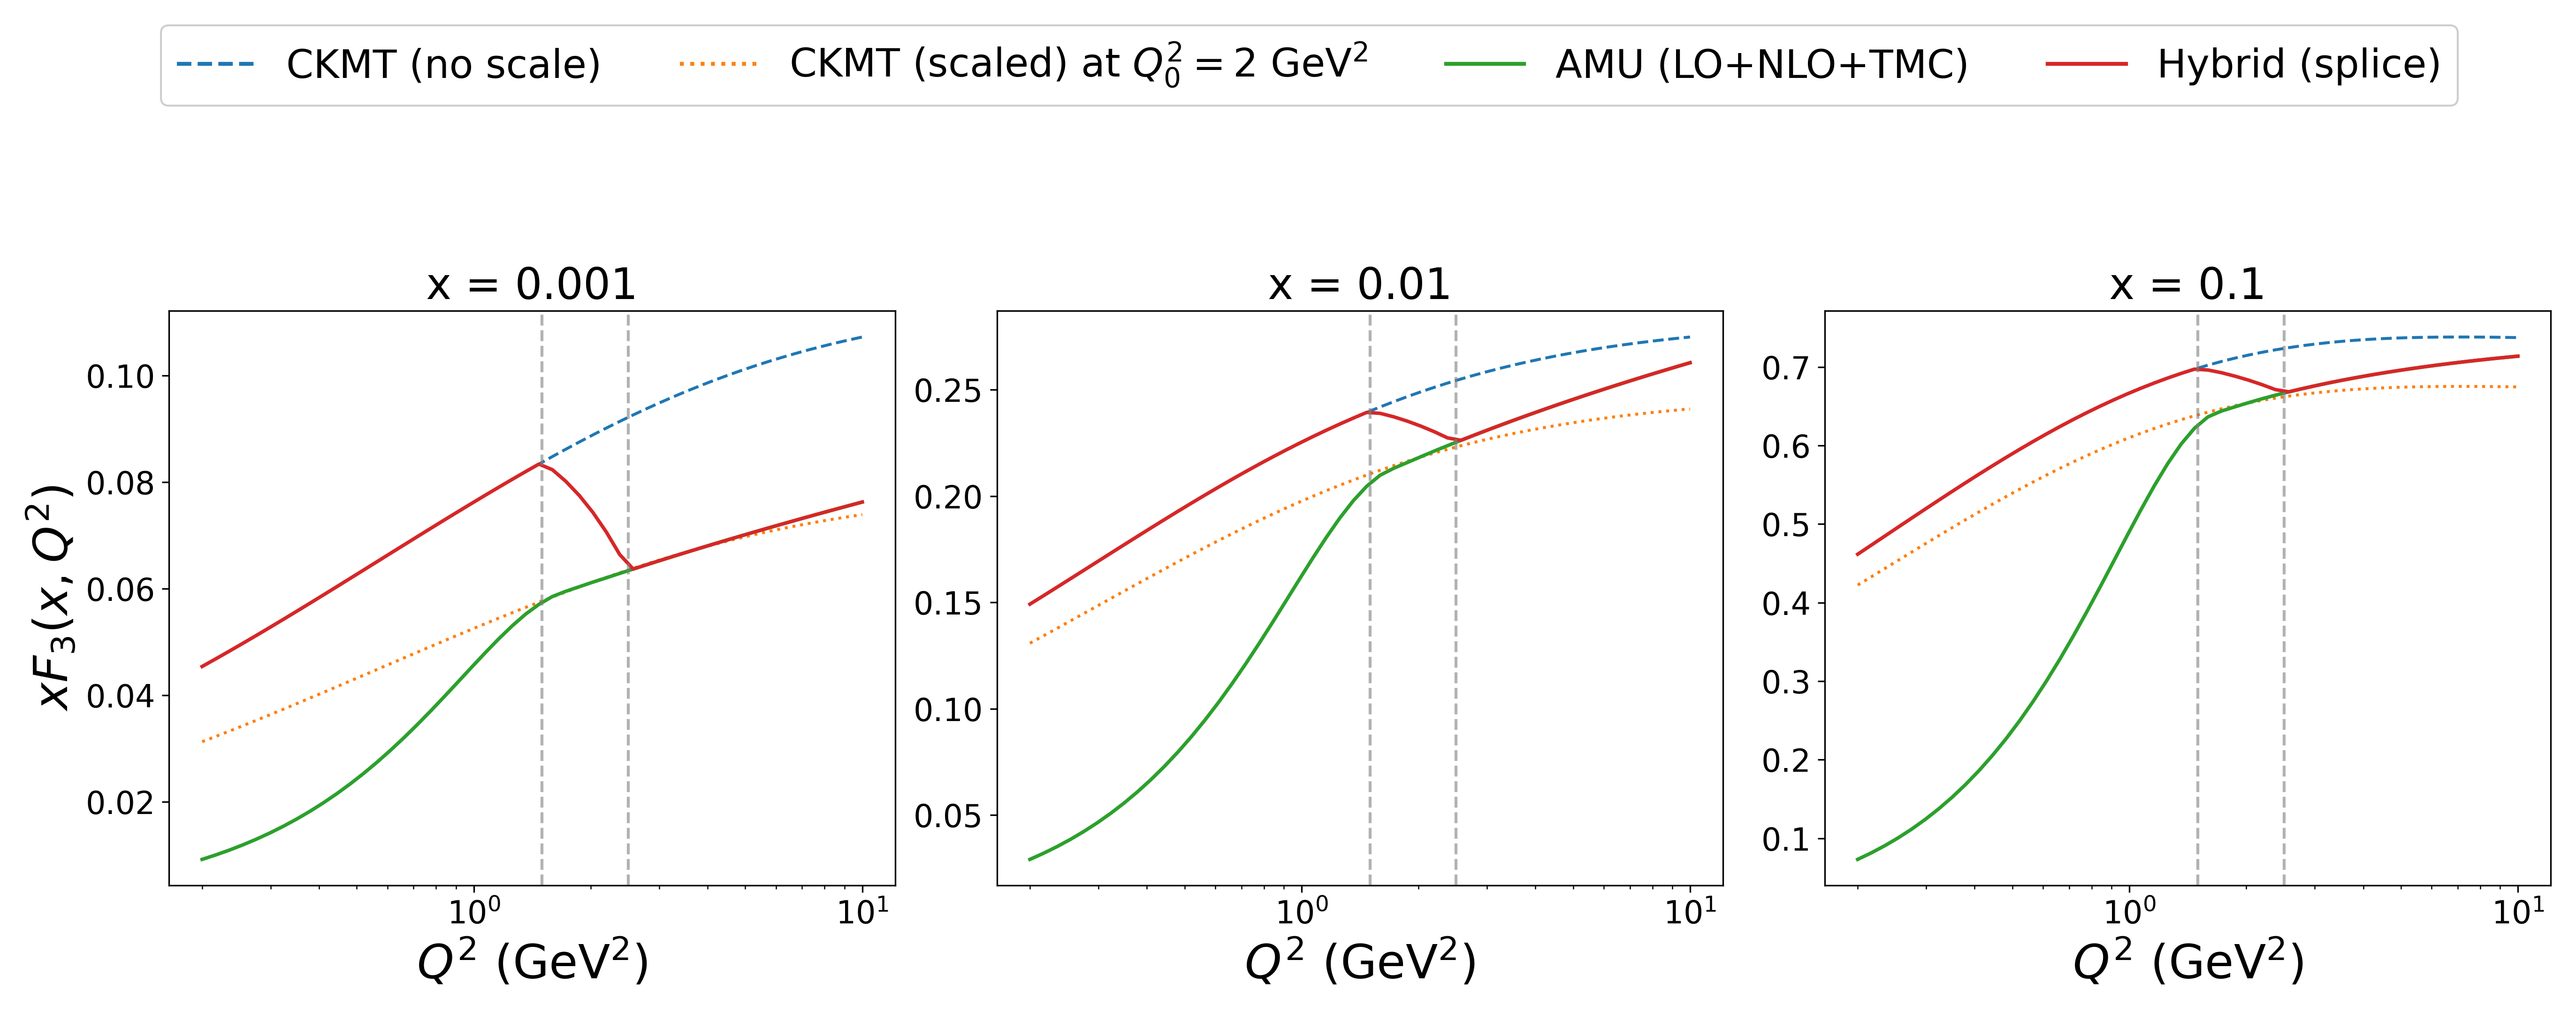
\includegraphics[width=0.88\textwidth]{slide_3panel_F3ckmt_amu_tmc.png}
  \captionof{figure}{$xF_3(x,Q^2)$ vs.\ $Q^2$ for the linear splice: unscaled CKMT
    (blue dashed), scaled CKMT (orange dotted), AMU with TMC (green solid), and the
    hybrid (red solid). The kink and slope discontinuity are most prominent at low~$x$.}
  \label{fig:xf3_matching}

  \vspace{0.35em}
  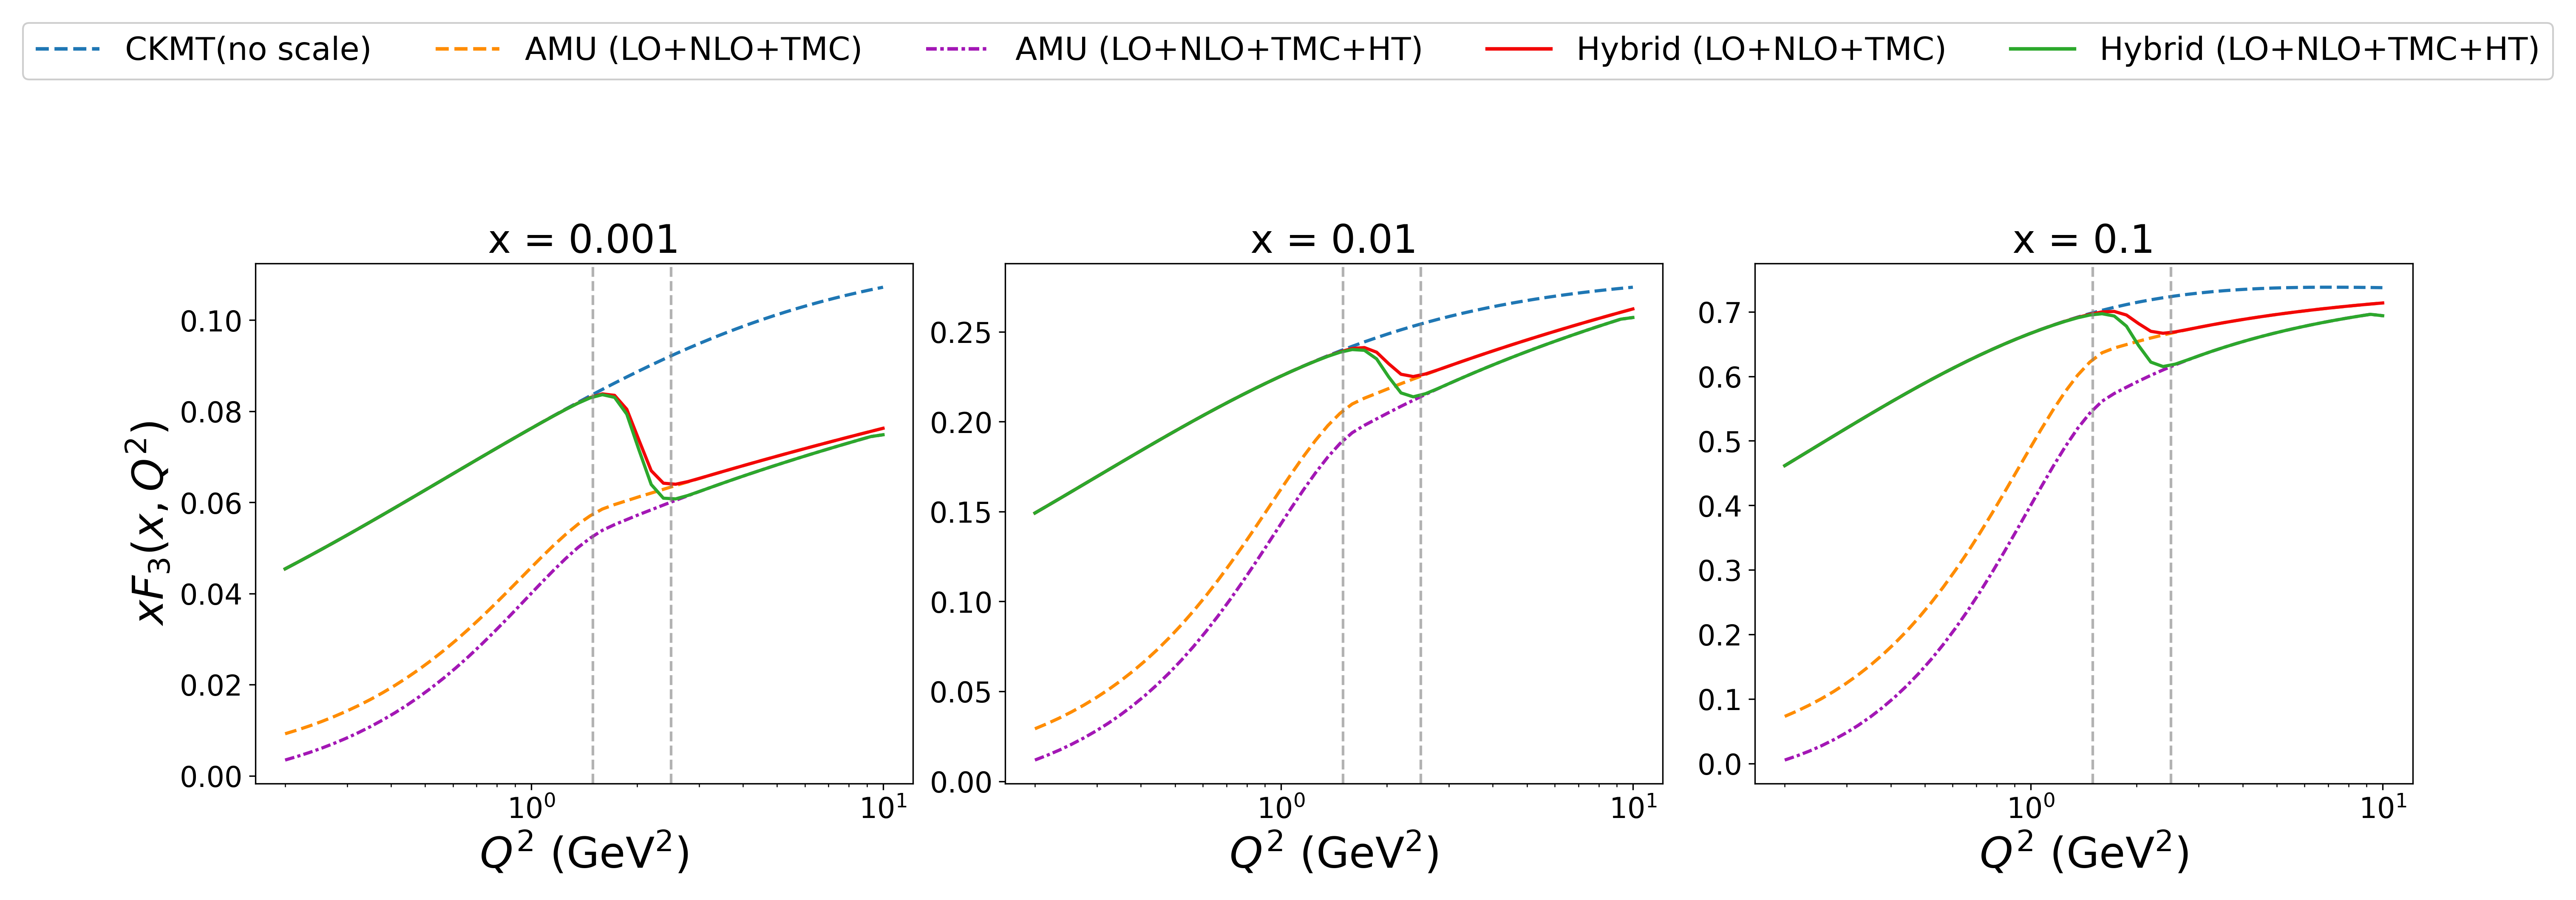
\includegraphics[width=0.88\textwidth]{panel_f3sigmoid_delta.25_tmc_ht.png}
  \captionof{figure}{$xF_3(x,Q^2)$ vs.\ $Q^2$ with smooth sigmoid matching
    ($\Delta=0.25$~GeV$^2$). Derivative continuity is restored, but the normalization
    offset leaves a non-monotonic dip; HT corrections deepen it slightly.}
  \label{fig:xf3_sigmoid}

  \vspace{0.35em}
  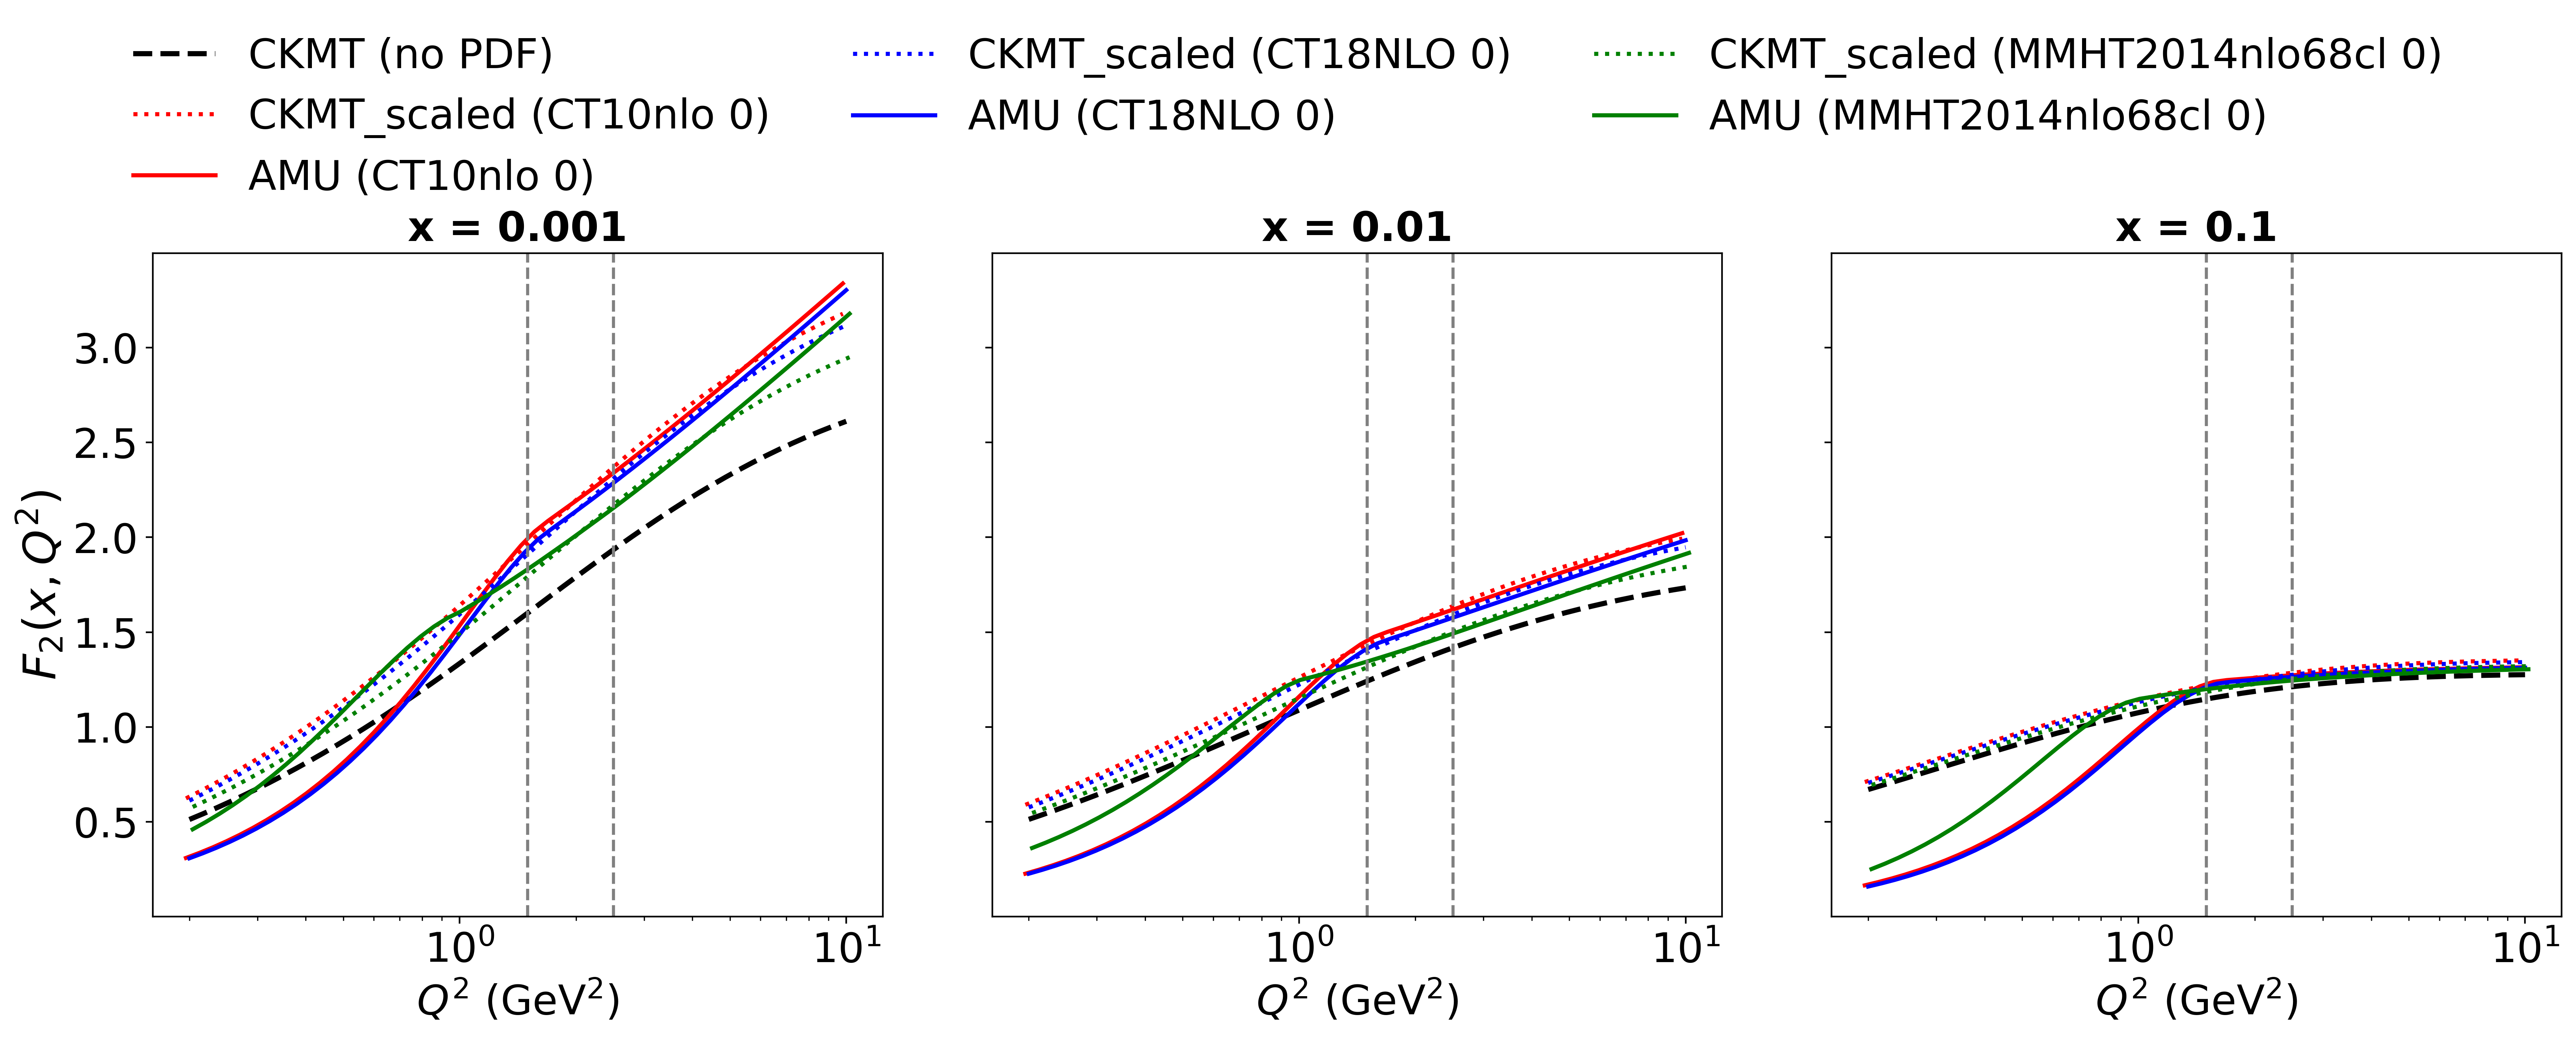
\includegraphics[width=0.48\textwidth]{Fig4a.png}\hfill
  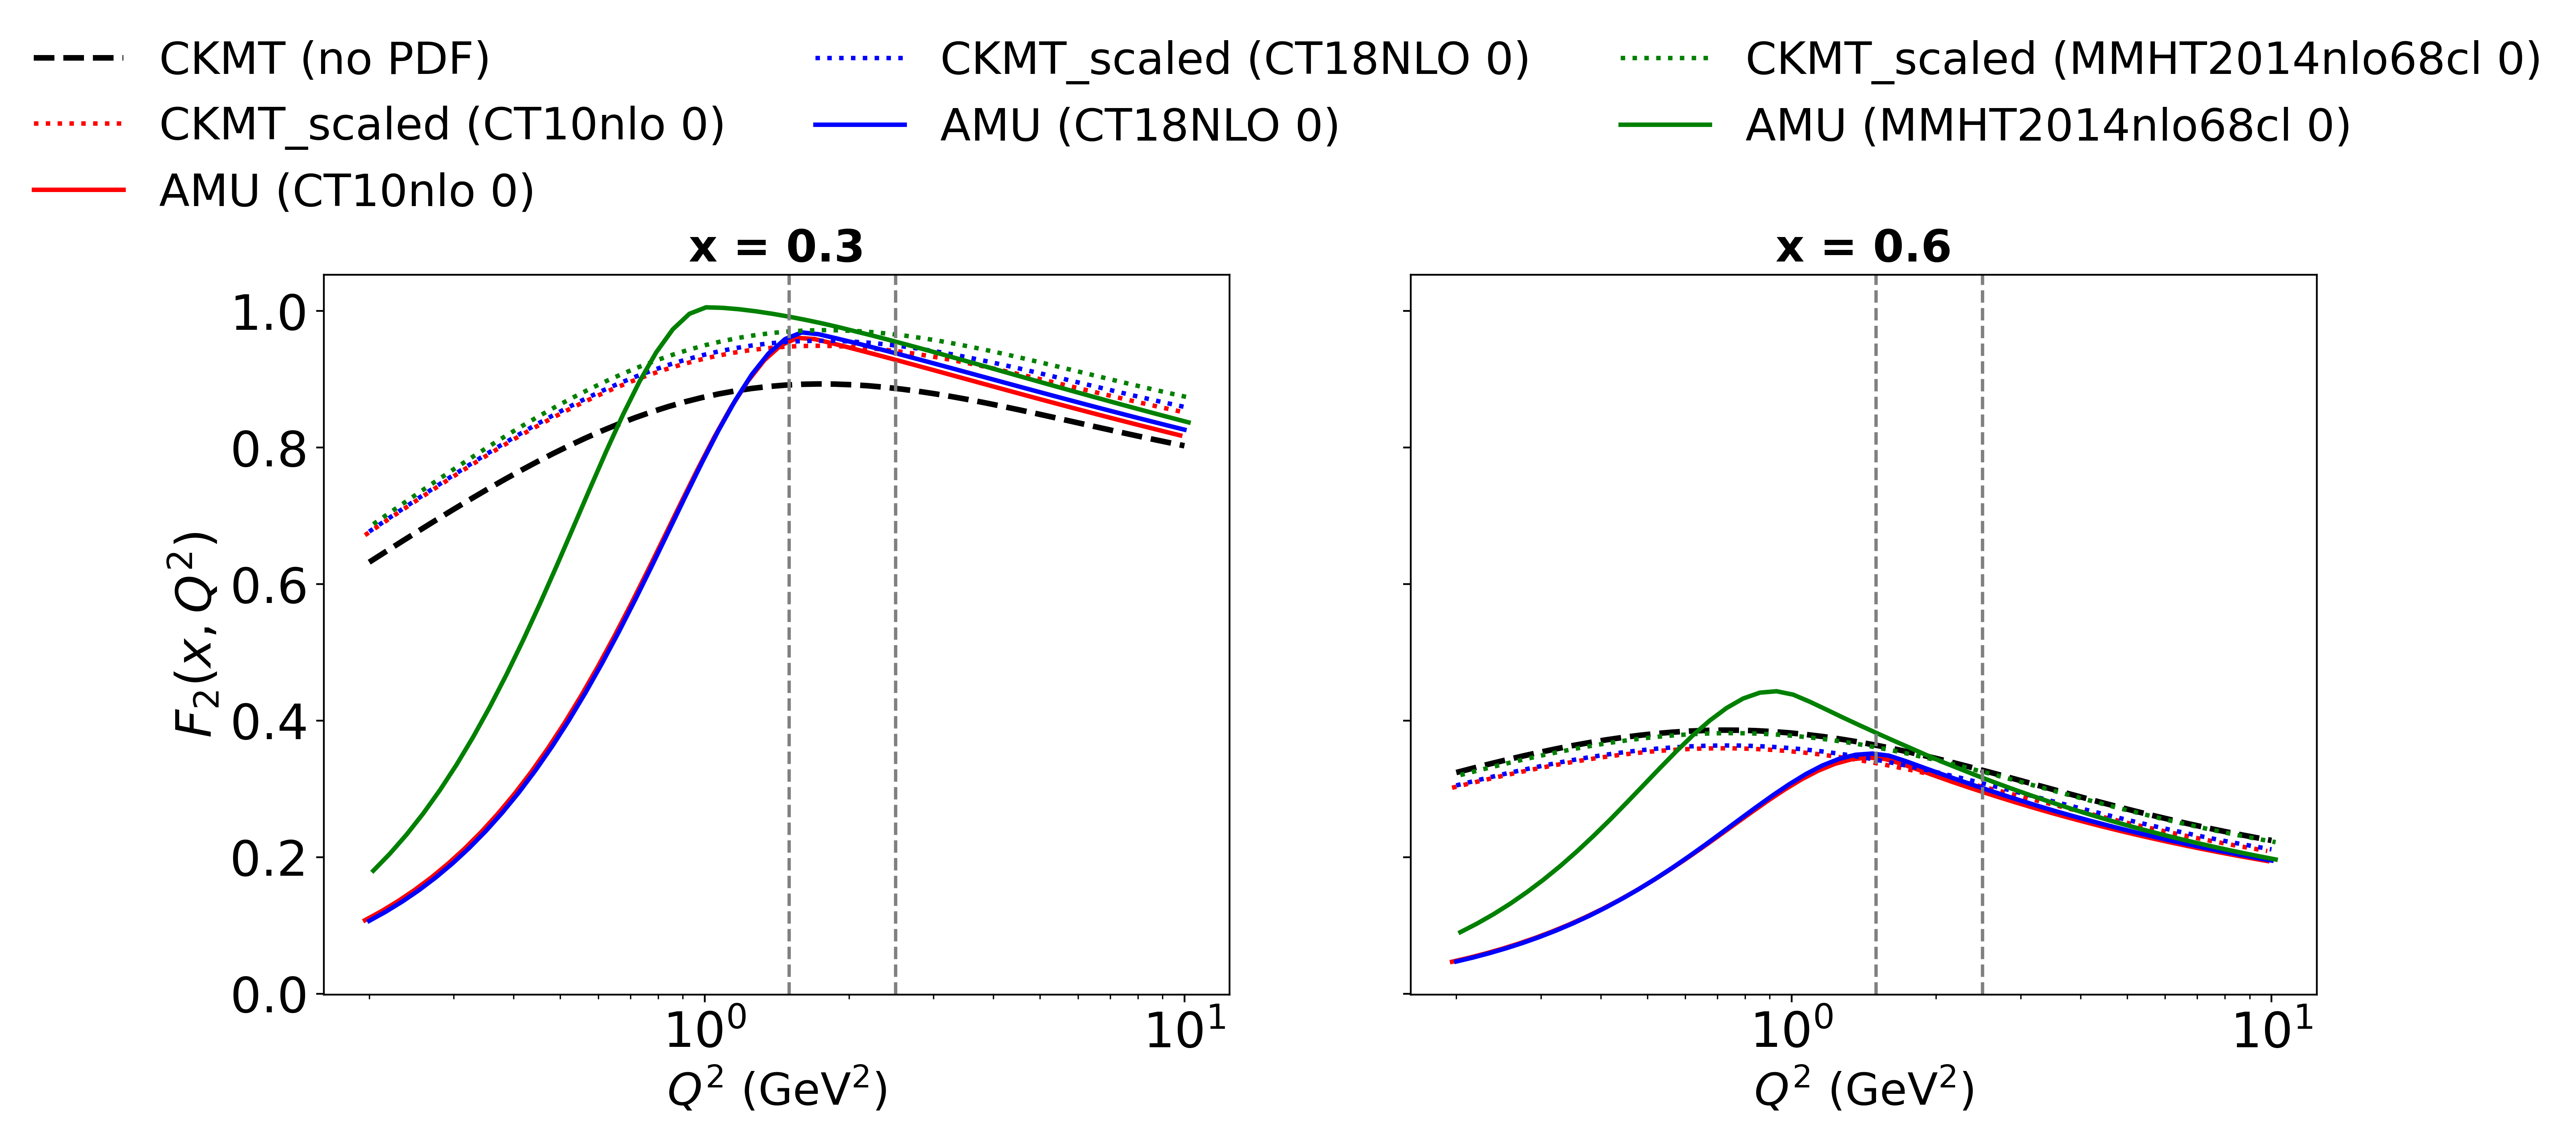
\includegraphics[width=0.48\textwidth]{Fig4b.png}
  \captionof{figure}{$F_2(x,Q^2)$ vs.\ $Q^2$ for CT10nlo, CT18NLO, and
    MMHT2014nlo68cl. The PDF spread is small at low~$x$ and larger at high~$x$.}
  \label{fig:pdf_sensitivity}
\end{figure*}



\subsection{PDF Sensitivity}

Figure~\ref{fig:pdf_sensitivity} shows $F_2$ for three PDF sets
(CT10nlo, CT18NLO, MMHT2014nlo68cl).
At low $x$ the sets converge before the splice window, leaving the
hybrid effectively PDF-independent in that region.
At high $x$ ($0.3$, $0.6$) the PDF spread is larger and extends
closer to $Q^2_0$, motivating a full PDF uncertainty quantification.

% ===================== SECTION 4 ================================
\section{Conclusions}
\label{sec:conc}

We have presented a hybrid framework for the charged-current weak
structure functions $F_2$ and $xF_3$ that bridges the
non-perturbative CKMT description at low $Q^2$ and the AMU
(NLO+TMC+HT) pQCD calculation at high $Q^2$:
\begin{enumerate}
  \item The optimal changeover scale is $Q^2_0 = 2.0$~GeV$^2$.
  \item Linear splicing produces visible kink artefacts for $xF_3$,
    most pronounced at low~$x$.
  \item Sigmoid weighting ($\Delta = 0.25$~GeV$^2$) restores derivative
    continuity, but an unphysical dip persists due to the normalization
    gap with unscaled CKMT, which is further accentuated by HT corrections.
  \item PDF sensitivity is significant at high~$x$ and low~$Q^2$, and
    vanishes above the matching scale.
\end{enumerate}

Future work will include validation against CCFR/NuTeV structure-function
data, extension to a wider range of nuclear targets, inclusion of
PCAC/axial contributions, and a full PDF uncertainty quantification.

% ===================== CONFLICT OF INTEREST ====================
\section*{Conflict of Interest}

The authors declare that they have no conflict of interest.
No for-profit product is discussed or implied in this article.

% ===================== REFERENCES ==============================
\begin{thebibliography}{99}
\small
\setlength{\itemsep}{1.5pt}
\setlength{\parskip}{0pt}

\bibitem{nuxsec}
  L. Alvarez-Ruso et al.\ (NuSTEC Collaboration),
  Prog.\ Part.\ Nucl.\ Phys.\ \textbf{100}, 1 (2018).
  \href{https://doi.org/10.1016/j.ppnp.2018.01.006}{doi:10.1016/j.ppnp.2018.01.006}

\bibitem{bloomgilman}
  E.~D. Bloom and F.~J. Gilman,
  Phys.\ Rev.\ Lett.\ \textbf{25}, 1140 (1970).
  \href{https://doi.org/10.1103/PhysRevLett.25.1140}{doi:10.1103/PhysRevLett.25.1140}

\bibitem{lalakulich}
  O. Lalakulich et al.,
  AIP Conf.\ Proc.\ \textbf{1189}, 276 (2009).
  \href{https://doi.org/10.1063/1.3274170}{doi:10.1063/1.3274170}

\bibitem{BY}
  A. Bodek and U.~K. Yang,
  Nucl.\ Phys.\ B Proc.\ Suppl.\ \textbf{112}, 70 (2002).
  \href{https://doi.org/10.1016/S0920-5632(02)01755-3}{doi:10.1016/S0920-5632(02)01755-3}

\bibitem{CKMT}
  A. Capella, A. Kaidalov, C. Merino, J. Tran Thanh Van,
  Phys.\ Lett.\ B \textbf{337}, 358 (1994).
  \href{https://doi.org/10.1016/0370-2693(94)90988-1}{doi:10.1016/0370-2693(94)90988-1}

\bibitem{jeong}
  Y.~S. Jeong and M.~H. Reno,
  Phys.\ Rev.\ D \textbf{108}, 113010 (2023).
  \href{https://doi.org/10.1103/PhysRevD.108.113010}{doi:10.1103/PhysRevD.108.113010}

\bibitem{CT10}
  H.-L. Lai et al.,
  Phys.\ Rev.\ D \textbf{82}, 074024 (2010).
  \href{https://doi.org/10.1103/PhysRevD.82.074024}{doi:10.1103/PhysRevD.82.074024}

\bibitem{Schienbein}
  I. Schienbein et al.,
  J.\ Phys.\ G \textbf{35}, 053101 (2008).
  \href{https://doi.org/10.1088/0954-3899/35/5/053101}{doi:10.1088/0954-3899/35/5/053101}

\bibitem{GENIE}
  C. Andreopoulos et al.,
  Nucl.\ Instrum.\ Meth.\ A \textbf{614}, 87 (2010).
  \href{https://doi.org/10.1016/j.nima.2009.12.009}{doi:10.1016/j.nima.2009.12.009}

\bibitem{NuWro}
  T. Golan, J.T. Sobczyk, J. Zmuda,
  Nucl.\ Phys.\ B Proc.\ Suppl.\ \textbf{229--232}, 499 (2012).
  \href{https://doi.org/10.1016/j.nuclphysbps.2012.09.136}{doi:10.1016/j.nuclphysbps.2012.09.136}

\bibitem{Stein1998}
  E. Stein et al.,
  Nucl.\ Phys.\ B \textbf{536}, 318 (1998).
  \href{https://doi.org/10.1016/S0550-3213(98)00589-3}{doi:10.1016/S0550-3213(98)00589-3}

\bibitem{Dasgupta1996}
  M. Dasgupta and B.~R. Webber,
  Phys.\ Lett.\ B \textbf{382}, 273 (1996).
  \href{https://doi.org/10.1016/0370-2693(96)00612-0}{doi:10.1016/0370-2693(96)00612-0}

\end{thebibliography}

\end{document}
